\documentclass[review,preprint,12pt]{elsarticle}
%\biboptions{numbers,super,comma}
\biboptions{round,authoryear,semicolon}
\renewcommand{\cite}{\citep} % make default citations parenthetical

\usepackage{amsmath}
\usepackage{amssymb}
\usepackage{amsthm}

\usepackage{graphicx}
%\usepackage{natbib}
\usepackage{caption}
\usepackage{subcaption}
\usepackage{hyperref}

\usepackage{color}
\usepackage{soul}

\usepackage{diagbox}

% Code from http://tex.stackexchange.com/questions/15735/adding-arrows-to-each-term-of-an-equation
\usepackage{tikz}
\usetikzlibrary{arrows}

\makeatletter

% Define how TiKZ will draw the nodes
\tikzset{mathterm/.style={draw=black,fill=white,rectangle,anchor=base}}
\tikzstyle{every picture}+=[remember picture]
\everymath{\displaystyle}

% Designate a term in a math environment to point to
% Syntax: \mathterm[node label]{some math}
\newcommand\mathterm[2][]{%
   \tikz [baseline] { \node [mathterm] (#1) {$#2$}; }}

% A command to draw an arrow from the current position to a labelled math term
% Default color=black, default arrow head=stealth
% Syntax: \indicate[color]{term to point to}[path options]
\newcommand\indicate[2][black]{%
   \tikz [baseline] \node [inner sep=0pt,anchor=base] (i#2) {\vphantom|};
   \@ifnextchar[{\@indicateopts{#1}{#2}}{\@indicatenoopts{#1}{#2}}}
\def\@indicatenoopts#1#2{%
   {\color{#1} \tikz[overlay] \path[line width=1pt,draw=#1,-stealth] (i#2) edge (#2);}}
\def\@indicateopts#1#2[#3]{%
   {\color{#1} \tikz[overlay] \path[line width=1pt,draw=#1,-stealth] (i#2) [#3] edge (#2);}}

\makeatother

%\biboptions{numbers,super,comma}

\newtheorem{theorem}{Theorem}[section]
\newtheorem{lemma}[theorem]{Lemma}

\theoremstyle{definition}
\newtheorem{definition}[theorem]{Definition}
\newtheorem{example}[theorem]{Example}
\newtheorem{xca}[theorem]{Exercise}

\theoremstyle{remark}
\newtheorem{remark}[theorem]{Remark}

\numberwithin{equation}{section}

%    Absolute value notation
%\newcommand{\abs}[1]{\lvert#1\rvert}

%    Blank box placeholder for figures (to avoid requiring any
%    particular graphics capabilities for printing this document).
\newcommand{\blankbox}[2]{%
  \parbox{\columnwidth}{\centering
%    Set fboxsep to 0 so that the actual size of the box will match the
%    given measurements more closely.
    \setlength{\fboxsep}{0pt}%
    \fbox{\raisebox{0pt}[#2]{\hspace{#1}}}%
  }%
}

\journal{Cell Systems}

\begin{document}

\begin{frontmatter}

\title{ %Exploiting redundancy in biological data to scale search tools with entropy \\
Entropy-scaling search of massive biological data}

%    Information for first author
\author[mitmath,mitcsail]{Y. William Yu\corref{co}}
%\ead{ywy@mit.edu}
\author[mitmath,mitcsail]{Noah M. Daniels\corref{co}}
%\ead{ndaniels@csail.mit.edu}
\author[mitcsail]{David C. Danko}
%\ead{dcdanko@mit.edu}
\author[mitmath,mitcsail]{\\Bonnie Berger\corref{correspond}}
\ead{bab@mit.edu}
%    Address of record for the research reported here
\cortext[co]{These authors contributed equally to this work.}
\cortext[correspond]{Corresponding author}
\address[mitmath]{Department of Mathematics, Massachusetts Institute of Technology, Cambridge, Massachusetts 02139}
\address[mitcsail]{Computer Science and AI Lab, Massachusetts Institute of Technology, Cambridge, Massachusetts 02139}

%\email{bab@mit.edu}

%    General info
%\subjclass[2010]{Primary 68W99}

%\date{September 23, 2014}

%\dedicatory{This paper is dedicated to our advisors.}

%\begin{keyword}
%Similarity search, approximate matching, entropy scaling algorithms
%\end{keyword}

\begin{abstract}
    \begin{itemize}
        \item While biological data sets are growing dramatically, they tend to exhibit low entropy
        \item We introduce a data structure that allows similarity search in time- and space-complexity asymptotically linear to entropy
        \item Using this data structure, we demonstrate substantial acceleration of search in the domains of metagenomics, chemogenomics, and protein structure search
    \end{itemize}
\noindent\unskip\textbf{eTOC Blurb}
\par\medskip\noindent\unskip\ignorespaces
Massive data sets in biological systems often exhibit high redundancy and thus low entropy.
We have developed a data structure for similarity search whose complexity scales nearly linearly in entropy.
This approach allows us to dramatically accelerate analytical tools drawn from genomics, small molecule search, and protein structure search.
\end{abstract}

\end{frontmatter}

%\maketitle
\section{Summary}
{ \bfseries
    The continual onslaught of new data from cell systems has forced upon scientists the fortunate problem of having too much data to analyze.
    Luckily, it turns out that many data sets exhibit well-defined structure that can be exploited for the design of 
smarter analysis tools.
    We introduce an entropy-scaling data structure---which given a low fractal dimension database, scales in both time and space with the entropy of that underlying database---to perform similarity search, a fundamental operation in data science.
    Using these ideas, we present accelerated versions of standard tools for use by practitioners in the three domains of metagenomics, high-throughput drug screening, and protein structure search, none of which have any loss in specificity or significant loss in sensitivity:
    CaBLASTX, 700x speedup of BLASTX with less than 5\% loss in sensitivity; Ammolite, \hl{??}x speedup of small molecule similarity search with \hl{??} loss in sensitivity; and, esFragBag, 10x speedup of FragBag with less than 0.2\% loss in sensitivity.

    Source code: \url{http://gems.csail.mit.edu}
}

\section{Introduction}
Throughout all areas of data science, scientists are being confronted by an 
explosion of data.
In many fields, this increase is exponential in nature, outpacing Moore's and Kryder's laws on the respective doublings of transistors on a chip and long-term data storage density \cite{kahn2011future}.
As such, the challenges posed by the massive influx of data cannot be solved by waiting for faster and larger capacity computers, but require instead the development of data structures and representations that exploit and simplify complexity in the data set.

Here, we focus on similarity search, where the task at hand is to find all entries in some database that are `similar', or approximate matches, to some query item.
Much like sorting is a primitive operation in computer science, similarity search is a fundamental operation in data science and lies at the heart of many other problems.
Traditionally, approximate matching has been studied primarily in the context of strings under edit distance metrics (e.g., for spell-checkers) \cite{ukkonen1985algorithms}.
However, similarity search has also demonstrated increasing importance in biological system domains, including local alignment of sequences \cite{altschul1990basic, kent2002blat}, chemical graphs \cite{schaeffer2007graph}, and protein structures \cite{budowski2010fragbag}.
%In recent years, however, similarity search has become increasingly important for other objects and distance functions (e.g., biological genomes and alignment scores, networks and the Jaccard index) [Altschul et al, 1990; Kent, 2002; Schaeffer, 2007].

As available data grows exponentially \cite{berger2013computational,yu2015quality} (e.g., genomic data in Figure S3), 
%move figure to supplement
algorithms that scale linearly with the amount of data no longer suffice.
The primary ways the literature addresses this problem (e.g.
locality sensitive hashing \cite{indyk1998approximate}, vector approximation \cite{ferhatosmanoglu2000vector}, space partitioning \cite{weber1998quantitative}) involve the construction of data structures that admit a more efficient search operation.
However, we note that as biological data increases, not only does the redundancy present in the data also increase~\cite{loh2012compressive}, but also internal structure (such as low fractal dimension) becomes apparent.
Existing general purpose methods do not explicitly exploit the particular internal structure of biological data to accelerate search.

In the specific context of local alignment in genomics, however, the emerging field of `compressive genomics' has shown that existing tools such as BLAST and BLAT can be compressively accelerated by taking advantage of high redundancy between related genomes using link pointers and edit scripts to a database of unique sequences \cite{loh2012compressive}.
Similar results have been demonstrated for local alignment in proteomics, using much the same strategies \cite{daniels2013compressive}.
Empirically, this compressive acceleration appears to scale almost linearly in the entropy of the database, often resulting in orders of magnitude better performance.

In this paper, we substantially generalize and formalize this approach by introducing the first mathematically rigorous class of entropy scaling data structures for similarity search: data structures that \textbf{provably} scale almost linearly in both time and space with the entropy of the database.
Specifically, if similarity is defined by a metric-like distance function (e.g., edit or Hamming distance) and the database exhibits both low `metric entropy' and `fractal dimension' (See Supplemental Methods: Theory), this data structure performs much better than na\"ive and even optimized methods.
This data structure allows for minimal (or even zero) loss in recall, coupled
with zero loss in specificity.
%We will define metric entropy and fractal dimension more precisely later, but intuitively, they are respectively measures of the total information content and scaling behavior of number of points contained in spheres of varying radii.
Although these entropy-scaling data structures can in principle be used to organize nearly any large data set for faster and more space-efficient analysis,
we demonstrate their utility on similarity search problems drawn from the three major biological ``big challenges of big data'': genomics, pharmaceuticals, and protein structure \cite{marx2013biology}.

\section{Results}
\subsection{Entropy-scaling data structure for similarity search}
\begin{figure}[btp]
    \centering
    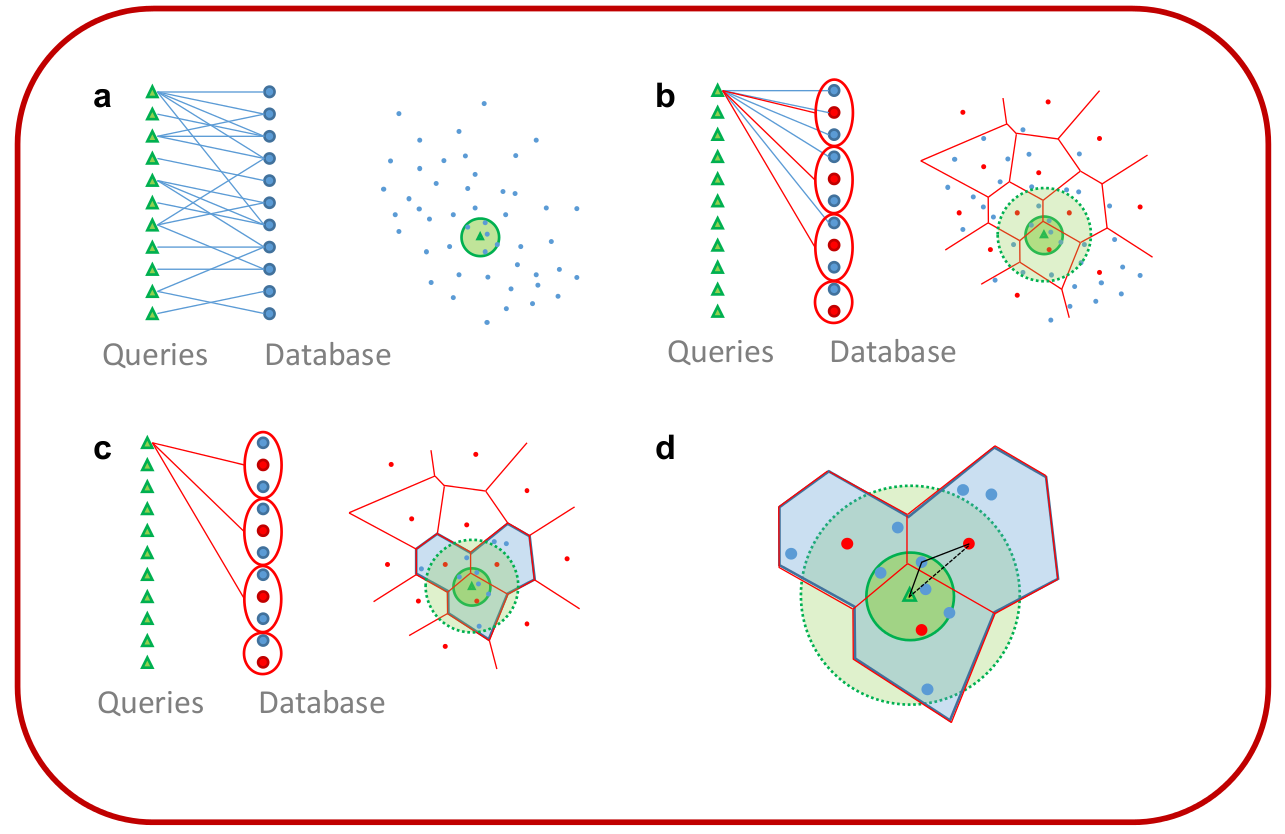
\includegraphics[width=1\textwidth]{assets/dataStructure.png}
    \caption{ Entropy-scaling data structure for similarity search. %
            (a) The na\"ive approach tests each query against each database entry to find entries within distance $r$ of the query (inside the small green disc). %
            (b) By selecting appropriate cluster centers with maximum radius $r_c$ to partition the database, we can (c) first do a coarse search to find all cluster centers within distance $r+r_c$ of a query (larger green disc), %
 and then the (d) triangle inequality guarantees that a fine search over all corresponding cluster entries (blue polygonal regions) will suffice.}
    \label{fig:dataStructure}
\end{figure}

%We present here an opportunistic data structure for similarity search that scales with the entropy of the underlying database.
In the following we consider entropy to be nearly synonymous with distance between points in a high-dimensional space.
For genomic sequences, this can be edit distance; for chemical graphs, maximum common subgraph size; and for general vectors, Euclidean or cosine distance.
We are interested in the similarity search problem of
finding all points in a set that are close to (i.e. similar to) the query point.
The basics of the data structure itself are presented in Figure \ref{fig:dataStructure}, but here we provide conceptual motivation.

Let us first consider what it means for a large biological data set, considered as points in a high-dimensional space, to be highly redundant.
Perhaps many of the points are exact duplicates; this easy scenario is trivially exploited by de-duplication and is already standard practice (e.g. the NR NCBI protein database \cite{pruitt2005ncbi}).
Or maybe the points mostly live on a low-dimensional subspace; statistical tools such as PCA (Principal Component Analysis) exploit this property in data analysis.
Furthermore, if the dimension of the subspace is sufficiently low,
it can be divided into cells, allowing quick similarity searches by looking only at nearby cells \cite{weber1998quantitative}.
However, when the dimensionality of the subspace increases, cell search time blows up exponentially; additionally, in sparse data sets, most of the cells will be empty, which wastes search time.
%Also, cell search performs poorly when each of the dimensions is small and discrete, as is the case with genomic sequences when we consider each position as a dimension and the four possible nucleotides as the possible locations along that axis.

\begin{figure}[btp]
    \centering
    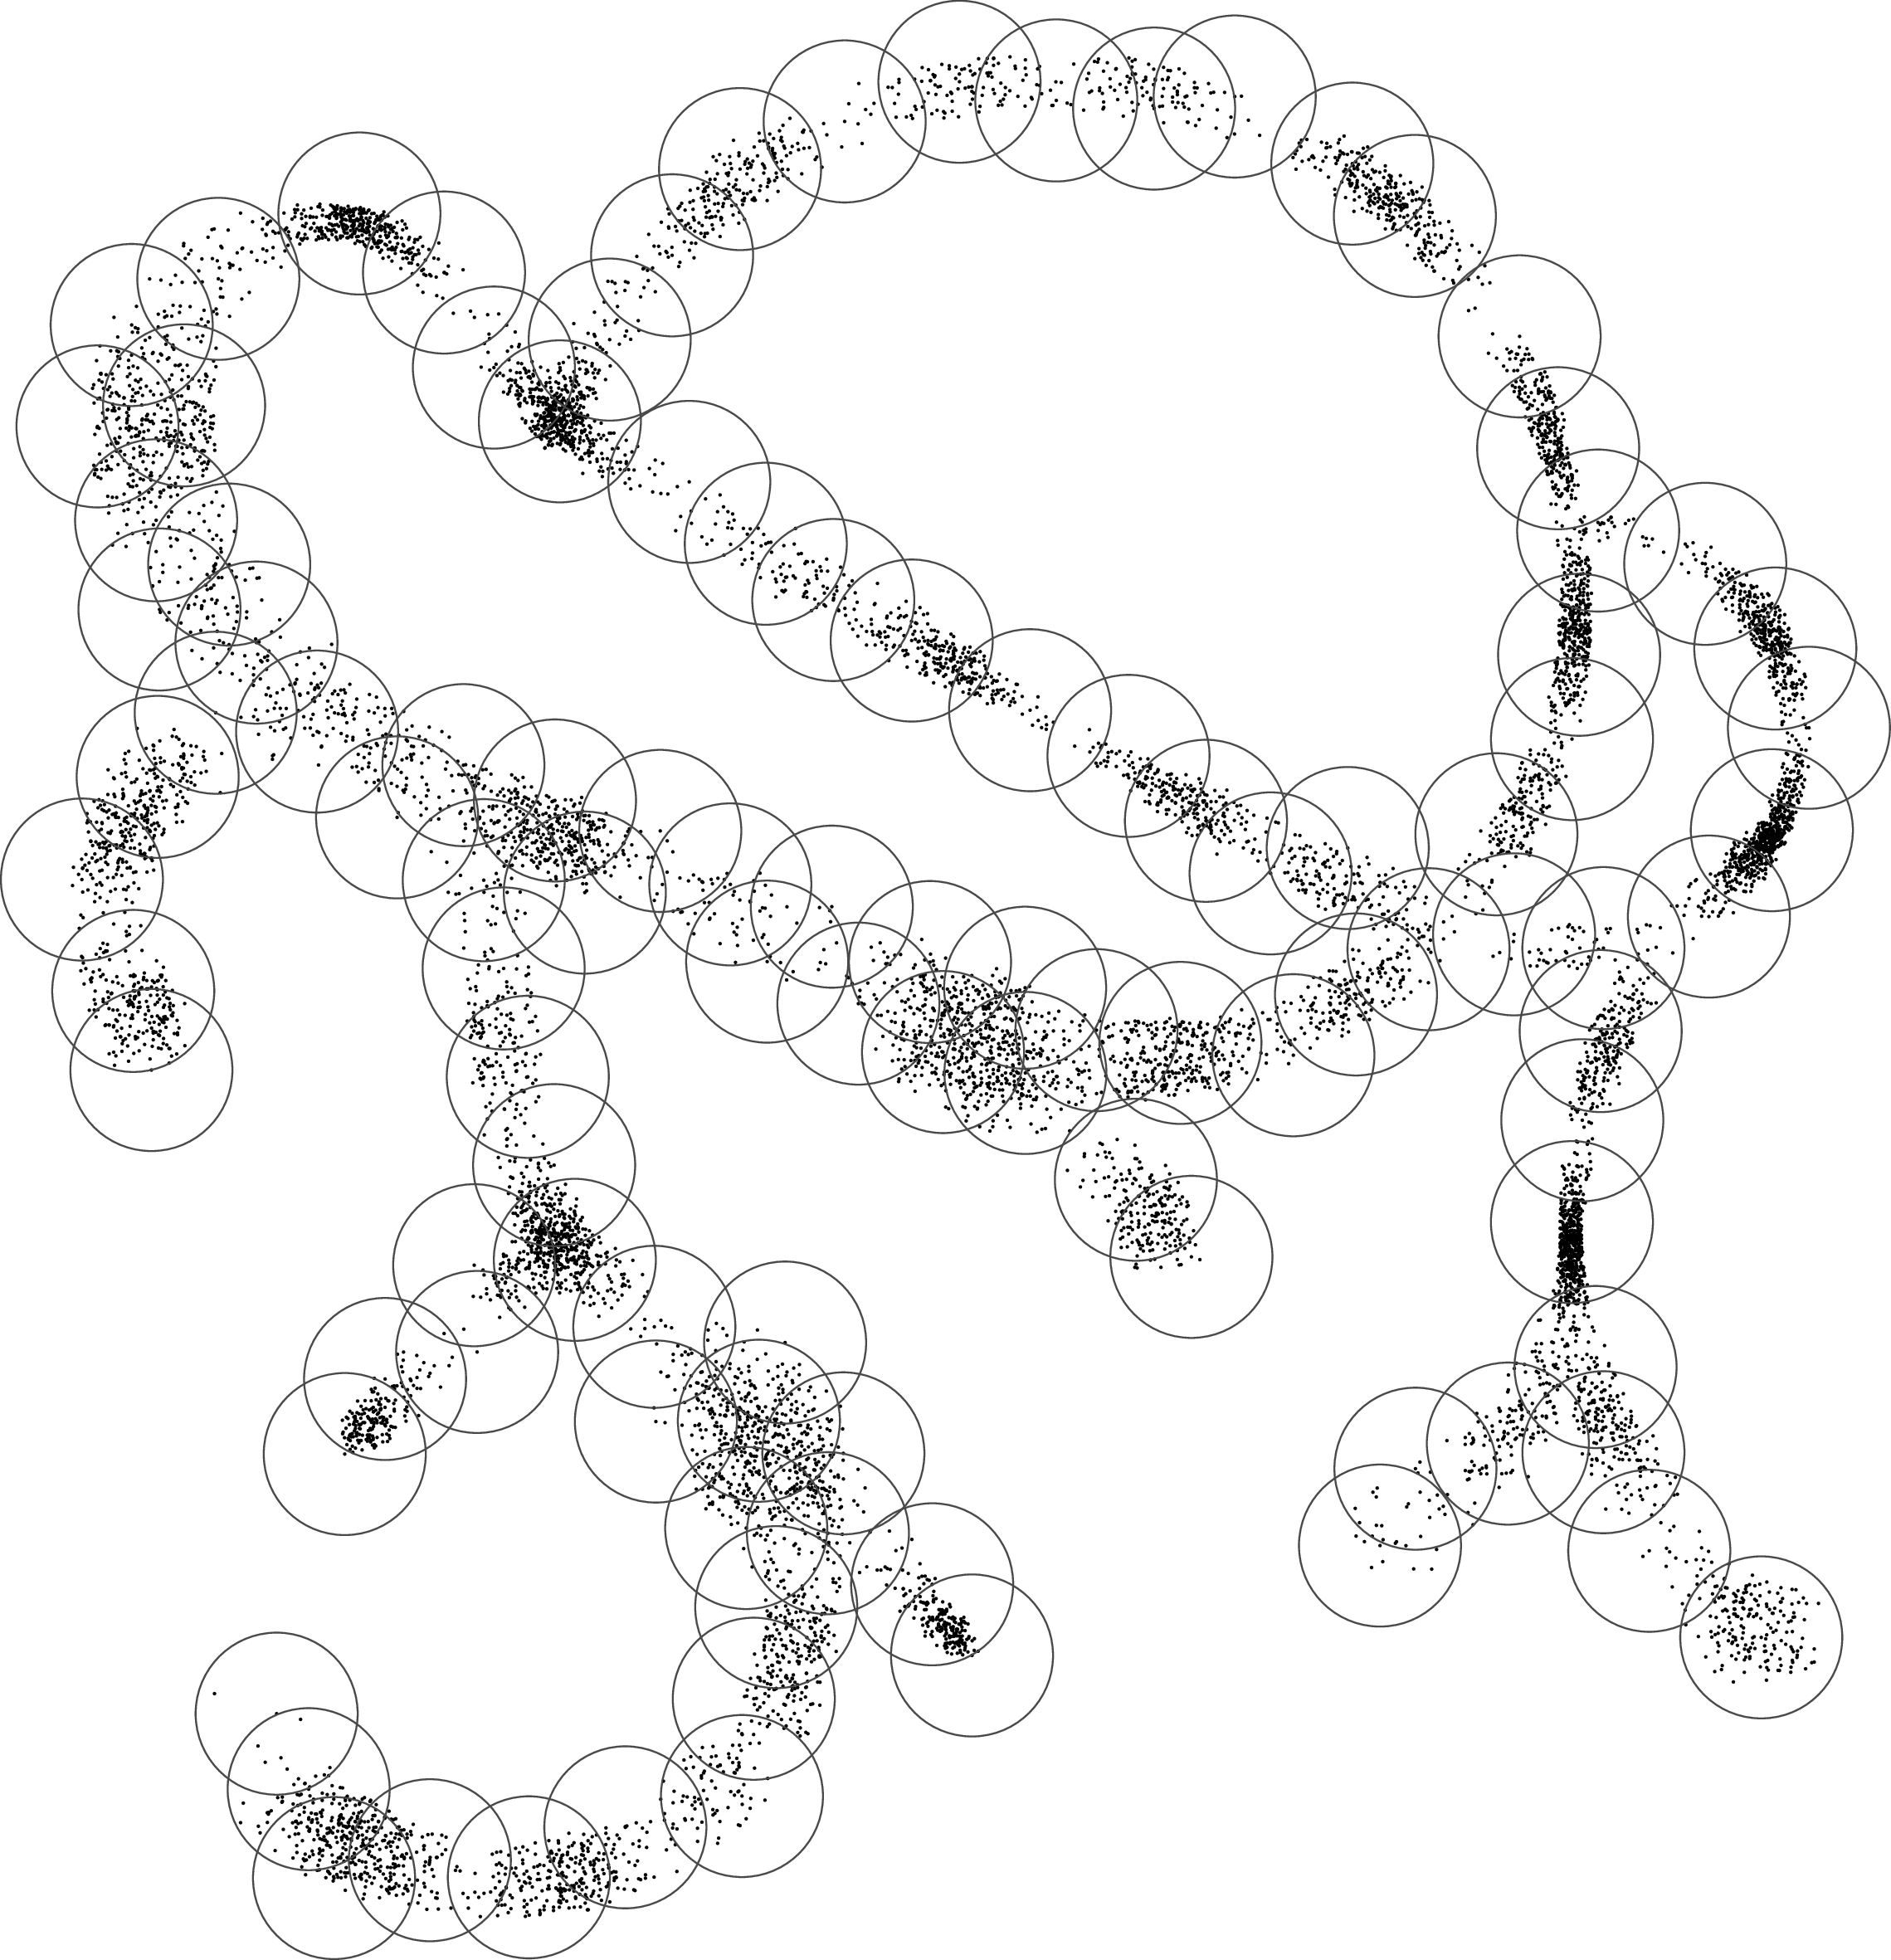
\includegraphics[width=0.8\textwidth]{assets/treepoints/treepoints2D_clusters.png}
    \caption{Cartoon depiction of points in an arbitrary high-dimensional space that live close to a 1D tree-like structure, as might arise from genomes generated by mutation and selection along an evolutionary tree of life. 
Although high-dimensional at a fine scale, at the coarser scale of covering spheres, the data cloud looks nearly 1-dimensional, which enables entropy-scaling of similarity search. The cluster center generation was performed using the same method we used for protein structure search.}
    \label{fig:tree}
\end{figure}
More importantly, biological data sets generally do not live in low-dimensional subspaces.
Consider the instructive case of genomes along an evolutionary Tree of Life (Figure \ref{fig:tree}).
Such a tree has many branches (plus admixture merges branches back together),
looks nearly 1-dimensional locally, but it is not globally.
Additionally, because of diffusion due to mutation, each of the branches is also ``thick'' (high-dimensional) when looked at closely.
%Figure 1b for illustration.
%Please look up Jinbo Xu and my work on Tree Decomposition in JACM.
% NMD: I'm familiar with TreePack, but not seeing how it's relevant.
Considering this example as a low-dimensional \textit{subspace}, as in PCA, is 
incorrect.

However, the local low-dimensionality can be exploited by looking on the right scales: a coarse scale in which the tree looks 1-dimensional locally and a fine scale where the branch width matters.
We cover the tree with spheres of radius $r_c$ on the order of the branch widths; these spheres determine our clusters, and the number of them is the metric entropy of the tree \cite{tao2008product}.
Because all the points within a sphere are close to each other, they are highly redundant and can be encoded in terms of one another, saving space in our representation.

By the triangle inequality, in order to search for all points within distance $r$ of a query we need only look in nearby spheres with centers within a distance $r+r_c$ of the query (Figure \ref{fig:dataStructure}d).
%ref Figure 1?.
However, because the spheres have radius comparable to branch width, the tree is locally 1-dimensional on the coarse scale---we will call this the fractal dimension $d=1$ of the tree at the scale $r_c$ \cite{falconer1990fractal}, where $r_c$ is essentially our ruler size.
Thus, increasing the search radius for coarse search only linearly increases the number of points that need to be searched in a fine search.

A similar analysis holds in the more general case.
Given a database with fractal dimension $d$ and metric entropy $k$ at the scale $r_c$, we show in the Supplemental Methods that the time-complexity of similarity search on database $D$ for query $q$ with radius $r$ is
\begin{gather}
    O\Bigg(
    \underbrace{k}_{\textrm{metric entropy}} +
    \overbrace{\left|B_D(q,r)\right|}^{\textrm{output size}}
    \underbrace{\left(\frac{r+2r_c}{r}\right)^d}_{\textrm{scaling factor}}
     \Bigg) .
\end{gather}
Thus, for small fractal dimension and output size, similarity search is asymptotically linear in metric entropy.
Additionally, because the search has to look at only a small subset of the clusters, the clusters can be stored in compressed form, and only decompressed as needed, giving space savings that also scale with entropy.
As an aside, note that the space-complexity actually scales with the sum of metric and information-theoretic entropy, rather than just metric entropy (See Supplemental Methods: Theory).
%Similarly, using these covering spheres, the database can be stored in a 
%compressed manner (see Supplemental Methods for further details).

We have presented the simplest such data to analyze for clarity of exposition.
However, real data is generally messier.
Sometimes the distance function is not a metric, so we lose the triangle inequality guarantee of 100\% sensitivity;
sometimes different distance functions can be used for the clustering versus search;
and sometimes even what counts as a distinct data point is not entirely clear without domain knowledge (for example, long genomic sequences might be better broken into shorter subsequences).

We show in the following that entropy-scaling data structures are robust to the variations that real data presents.
Through the diversity of the applications we explore in this paper, we demonstrate that the general scheme works for massively accelerating similarity search in a set of different contexts.
These applications are enabled by augmenting the data structure with domain-specific distance functions in different stages of the algorithm, as well as preprocessing to take advantage of domain-specific knowledge.
We expect that so long as the data set exhibits both low entropy (many items are similar to one another, which is nearly always the case when the query is a similarity search) and low fractal dimension (the data set has some much simpler structure generating it, such as an evolutionary tree, as often seems to be the case in biology), our entropy-scaling data structure has the potential to achieve massive speedup over more naive methods and significant speedup over even other highly optimized methods.

\subsection{Application to Metagenomics}

Metagenomics is the study of genomic data sequenced directly from environmental
samples.
It has led to improved understanding of how ecosystems recover
from environmental damage~\cite{tyson2004community} and how the human gut responds 
to diet
and infection~\cite{david2014host}.
Metagenomics has even provided some surprising insights into disorders 
such as Autism Spectrum Disorder~\cite{macfabe2012short}.

BLASTX~\cite{altschul1990basic} is widely used in metagenomics to map
reads to protein databases such as KEGG~\cite{kanehisa2000kegg} and NCBI's 
NR~\cite{sayers2011database}.
This mapping is additionally used as a primitive in pipelines such as MetaPhlAn~\cite{segata2012metagenomic}, 
PICRUSt~\cite{langille2013predictive}, and MEGAN~\cite{huson2011integrative} to
determine the microbial composition of a sequenced sample.
Unfortunately, BLASTX's run time requirements scale linearly with the size of the 
full read dataset, and each year require exponentially more runtime to process 
the exponentially growing read data. 
These computational challenges are at present a barrier to widespread use of 
metagenomic data throughout biotechnology, which impacts genomic medicine and 
environmental genomics~\cite{frank2008gastrointestinal}.
For example, \citet{mackelprang2011metagenomic} reported that using BLASTX to map 246
million reads against KEGG required 800,000 CPU hours at a supercomputing 
center.

Although this is a problem already for major research centers, it is especially
limiting for on-site analyses in more remote locations.
In surveying the 2014 Ebola outbreak, scientists physically shipped samples on 
dry ice to Harvard for sequencing and analysis \cite{gire2014genomic}.
Even as sequencers become more mobile, lack of fast Internet connections in remote
areas can make it impossible to centralize and expediate processing (viz.: the cloud);
local processing on resource-constrained machines remains essential.
Thus, a better scaling and accurate version of BLASTX promises the possibility of not only faster computing for
large research centers, but also of enabling the novel workflow of
entirely on-site local sequencing and metagenomic analyses.

We have applied our entropy-scaling data structure to the problem of 
metagenomic search, and demonstrate caBLASTX, a method whose software 
implementation provides an acceleration of BLASTX by a factor of up 
to 673.
This application illustrates the potential of entropy-scaling data structures, while
providing a useful tool for metagenomic research.

CaBLASTX is useful for two of the most common metagenomic analysis tasks. 
The first of these is mapping short nucleotide reads (generated by next-generation sequencing (NGS) technology) to a protein database,
while the second is mapping assembled or partially-assembled
nucleotide sequences onto a protein database.
In the former instance, there is typically high coverage of the metagenomes
being sequenced, ranging from 30x to 200x coverage.
CaBLASTX takes advantage of this redundancy
by clustering the read set as well, obtaining an additional speed gain that is
proportional to the amount of redundancy in the read data.
We note that this query-side clustering is not part of the entropy-scaling
framework as described, and as the run-time cost of clustering queries cannot
be amortized over future queries,
%BAB Maybe it can?
we expect this enhancement to provide a 
constant factor improvement.
%BAB why so?

To evaluate the run-time performance of caBLASTX, we tested it against
BLASTX as well as RapSearch2~\cite{zhao2012rapsearch2} and the recently-released
Diamond~\cite{buchfink2014fast}, and found substantial runtime improvements 
(although similar to Diamond) at significantly greater accuracy (Table~\ref{mgspeed}).
%BAB Can we show how the greater accuracy could be important?  For instance, I have 
% a SN article saying how two metagenome processing centers gave completely 
% different results.
%BAB Move next sentence to Supplementary results-- a detail?
%BAB We filtered out reads starting or ending with 10 or more no-calls ('N').
The running time for BLASTX was 14,423 minutes, 
while caBLASTX took 21 minutes, a speedup of 673x.

CaBLASTX also sped up BLASTX in aligning assemblies thought to be exons to a protein
database, in which case metagenomic reads have already been 
%BAB mostly?
assembled (Table~\ref{mgspeed}).
We benchmarked caBLASTX vs. BLASTX on a dataset consisting of 22,778 assemblies
from human gut microbiota, 3.1 megabases in total, searching against the NCBI's
``NR'' non-redundant protein database from September, 2014.
The running time of BLASTX was 3235 minutes, compared to 123 minutes for 
caBLASTX, a speedup of 26.3.
In this instance, the query-side clustering of caBLASTX is not applicable, so
the performance gains are more modest.
For both NGS reads and assemblies, Diamond had slightly faster running time than caBLASTX, albeit at the expense of accuracy, while RapSearch2 was slower.
% BAB: this makes more sense when you combine Tables 1 and 2.


% BAB: combine tables: Table 1 upper and accuracy table 2 lower
\begin{table}
\caption{Running time of BLASTX, caBLASTX, RapSearch2, and Diamond. All runtime in seconds.\label{mgspeed}}
\begin{tabular}{ccccc}
\hline
dataset & BLASTX & caBLASTX & RapSearch2 & Diamond \\
\hline
NGS reads (sec) & 14423 & 21 & 51 & 13 \\
\hline
assemblies (sec) & 3235 & 123 & 194 & 50 \\
\hline
\end{tabular}
\end{table}

% BAB: no indent--try to combine in one large table. With bold line dividing them. Just list BLASTX accuracy as 100%.
\begin{table}
\caption{Accuracy of caBLASTX, RapSearch2, and Diamond.\label{mgacc}}
\begin{tabular}{cccc}
\hline
dataset & caBLASTX & RapSearch2 & Diamond \\
\hline
NGS reads (sec) & 95.7\% & 79.5\% & 76.9\% \\
\hline
assemblies (sec) & 99.2\% & 87.7\% & 91.0\% \\
\hline
\end{tabular}
\end{table}

% BAB: table 1, lower
As shown in Table~\ref{mgacc}, on the metagenomic assemblies, where query-side 
% BAB: This implies query-side compression greatly reduces accuracy when it is really that these are protein sequences that are easy to assemble.  Address in discussion or make clearer here.
compression was not performed, caBLASTX achieves substantially better accuracy
than other methods: caBLASTX achieves 99.2\% accuracy on assemblies and 95.7\% 
accuracy even on the raw reads.
Experiments validating accuracy treated BLASTX as a gold standard. 
Since caBLASTX accelerates BLASTX
using entropy-scaling techniques, false positives with respect to BLASTX are 
not possible, but false negatives certainly are.
We evaluated the hits from BLASTX and caBLASTX on the same human gut
assemblies and raw reads used for benchmarking, in order to evaluate the accuracy when
query-side compression is not used.
As false positive hits with respect to BLASTX are not possible, we report as 
accuracy the fraction of BLASTX hits that are also returned by caBLASTX.
We note that due to query-side compression, the output order from caBLASTX 
typically does not match that of BLASTX.

While Diamond is somewhat faster than caBLASTX, it achieves this speed at the
expense of some accuracy, particularly on raw reads.
% BAB: how about space?
Moreover, caBLASTX actually accelerates standard BLASTX itself, and allows the
user to pass arbitrary parameters to the underlying BLASTX during fine search.
Thus, caBLASTX may be suitable to a wider variety of existing analysis 
pipelines.
% BAB: Maybe move this entire end of paragraph to Discussion and reverse in the context of entropy scaling speedup and accuracy.
It may be possible to apply entropy-scaling data
structures to Diamond itself, achieving even greater speed gains.
Of course, the accuracy of such an approach would still be limited by Diamond; 
% BAB: Following clause: main point in Discussion and use Diamond as an example.
entropy-scaling data structures cannot themselves improve accuracy,
except by virtue of making computationally expensive analyses more tractable.

\subsection{Application to High-throughput Drug Screening}

In the field of drug discovery and drug repurposing, prediction of biologically 
active compounds is a critical task. 
Computational high-throughput screening can eliminate many compounds from 
wet-lab consideration, but even this screening can be computationally 
intensive, and thus time-consuming.
PubChem~\cite{bolton2008pubchem} is a repository of molecular compound 
structures, 
which has grown greatly since 2008. 
In July, 2007, Pubchem contained 10.3 million compounds.
In October, 2013, PubChem contained roughly 47 million compounds, while
in December, 2014 it contained 61.3 million compounds.

We introduce Ammolite, a framework for clustering molecular databases that use the 
popular SDF molecular structure format, such as PubChem, and for quickly searching for 
similar molecular structures in compressed space.
We designed this compression and search framework around one of the standard 
techniques for high-throughput screening of potential drug compounds, the use 
of maximum common subgraph (MCS) to identify similar motifs among molecules \cite{cao2008maximum, rahman2009small}.
% BAB: reverse last two sentences if we get better speedup.
Ammolite demonstrates that entropy scaling methods can be extended to data types that are not inherently sequence based.
Ammolite is a practical 
tool that provides ~4x speed-up with greater than 95\% accuracy compared to the popular SMSD~\cite{rahman2009small}.

MCS based search of molecule databases typically matches pairs of molecules by 
their overlap coefficients. However, the overlap coefficient of two molecules is not a 
metric.
Molecules with a high overlap coefficient may be globally dissimilar if the 
larger molecule contains a significant subgraph of the smaller molecule.
Thus, overlap coefficient is desirable for identifying relevant structures in a 
molecule database, despite its not upholding the triangle inequality, in 
contrast to distance metrics such as graph distance \cite{bunke1998graph}.
% BAB: We never said why caBLASTx distance didn't have metric entropy. this sentence makes it sound that we have this framework, but it doesn't apply to real problems.
As with caBLASTX (which uses the non-metric distance of E-values), a more mathematically satisfying distance function must give 
way to one that has more meaning in the domain of interest; regardless, the
entropy-scaling still applies.

To compress a molecule database, we project the space of small molecules onto a subspace by removing nodes and edges that do not participate in simple cycles.
Clusters are exactly pre-images of of this projection operator (i.e. all molecules that are isomorphic after simplification form a cluster).
Coarse search is performed by finding the MCS on this much smaller projection subspace. This increases speed both by reducing the required number of MCS operations 
and by reducing the time required for each MCS operation, which scales with the size of the molecule.

\hl{Benchmarking paragraph(s)}


% BAB: reverse with actual results--positive things first!
\hl{Did not compare against CDK MCS algorithm because already done by [et al, Thornton] and did not compare against FMCS [Cao, et al] because 100 slower}

\hl{Validation paragraph(s)}

\hl{Typical workflow medicinal chemist using SMSD has week of downtime. With ours, weekend only. Need citesi (otherwise hypothetical).}

\subsection{Application to Protein Structure Search}

The relationship between protein structure and function has been a subject of intense study for decades,
and this strong link has been used for the prediction of function from structure \cite{hegyi1999relationship}.
Specifically, given a protein of solved (or predicted) structure but unknown function, the efficient identification
of structurally similar proteins in the Protein Data Bank is critical to function prediction.
Relatedly, finding structural neighbors can also give insight into the evolutionary origins of proteins of interest.

One approach to finding structural neighbors is to attempt to align the query protein to all the entries in the Protein Data Bank (PDB) using a structural aligner (e.g. STRUCTAL \cite{subbiah1993structural}, ICE \cite{shindyalov1998protein}, or Matt \cite{menke2008matt}).
However, performing a full alignment against every entry in the PDB is prohibitively expensive, especially as the database grows.
Alternately, the approach we use here is the one introduced by FragBag~\cite{budowski2010fragbag}, which describes each protein as a
`bag of fragments,' where each fragment is a small structural motif.
By directly applying our entropy scaling data structure without any additional augmentation, esFragBag (entropy scaling FragBag) is able to achieve a 2-30x speedup of the highly-optimized FragBag with less than 0.2\% loss in sensitivity and no loss in specificity.

For this last example, we intentionally approach the application of entropy-scaling data structures to FragBag in a blind manner,
without using any domain-specific knowledge.
Instead, we use the very same representation (bag of fragments) and distance functions (Euclidean and cosine distances)
as FragBag, coupled with a greedy k-centers algorithm to generate the clustered representation.
Note that this is in stark contrast to caBLASTX and Ammolite, which both exploit domain knowledge to further improve performance.
Thus, esFragBag only involves grafting new database generation and similarity search functions onto an existing codebase.

We explore the increases in speed resulting from applying the entropy-scaling data structure for both Euclidean and cosine distances (Figure \ref{fig:fragbag}).
Naturally, as search radii increases, the coarse search expands to encompass the entire database; to fully explore parameters, we make certain to increase search radii until the acceleration effect entirely disappeared.
Additionally, we explore the effect of using different maximum cluster radii and several different query proteins.

For cosine distance, we generated databases with maximum cluster radii of 0.1, 0.2, 0.3, 0.4, and 0.5.
Then, for each query protein from the set \{\texttt{4rhv}, \texttt{1ake}, \texttt{1bmf}, \texttt{1rbp}, \texttt{1b7t}\} (identified by PDB IDs), we ran both naive and accelerated similarity searches with radii of $0.02i, \forall i \in \{0,\ldots,49\}$.
This was repeated 5 times for each measurement, and the ratio of average accelerated vs naive times is shown in Figure \ref{fig:fragbag_cosine}.

For euclidean distance, we generated databases with maximum cluster radii of 10, 20, 25, 50, and 100.
Again, for each query protein drawn from the same set, we compared the average over 5 runs of the ratio of average accelerated vs naive times (Figure \ref{fig:fragbag_euclid}).

As expected, the acceleration is highly dependent on both the search radius $r$ and the maximum cluster radius $r_c$.
Additionally, the query protein also makes a major difference in the results.
We suspect that this is due to the geometry of protein fragment frequency space being very `spiky' and `star-like'.
Proteins that are near the core (and thus similar to many other proteins) show very little acceleration when our data structure is used because the majority of the database is nearby, whereas proteins in the periphery have fewer neighbors and are thus found much more quickly.
Changing the maximum cluster radius effectively makes more proteins peripheral proteins, but at the cost of overall acceleration.

Naturally, as the search radius expands, it quickly becomes necessary to compare against nearly the entire database, destroying any acceleration.
For the cosine space in particular, note that the maximum distance between any two points is $1$, so once the coarse search radius of $r+r_c >= 1.0$, there cannot ever be any acceleration as the fine search encompasses the entire database.
Similarly, once the coarse search encompasses all (or nearly all) the clusters in Euclidean space, the acceleration diminishes to 1x, and the overhead costs make the entropy scaling data structure perform worse than a na\"ive search.
However, as we are most interested in proteins that are very similar to the query, the low-radius behavior is of primary interest.
In the low-radius regime, esFragBag demonstrates varying though substantial acceleration (2x-30x, averaging >10x for both distance functions for the proteins chosen) over FragBag.

Additionally, it is instructive to note that because of the very different geometries of euclidean vs cosine space, acceleration varies tremendously for some proteins, such as \texttt{4rhv} and \texttt{1bmf}, which display nearly opposite behaviors.
Whereas there is nearly 30x acceleration for \texttt{4rhv} in cosine space for low radius, and the same for \texttt{1bmf} in euclidean space, neither achieves better than $\sim$ 2.5x acceleration in the other space.

\begin{figure}[tbp]
    \centering
    \begin{subfigure}[b]{0.40\textwidth}
        \caption{Cosine distance}
        \label{fig:fragbag_cosine}
        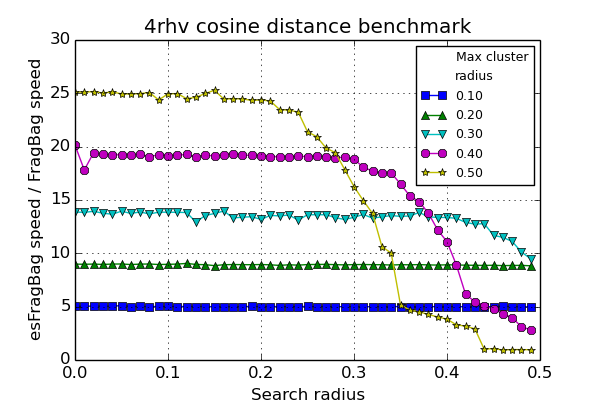
\includegraphics[width=1\textwidth]{assets/4rhv_cosine.png}
    \end{subfigure}%
    \begin{subfigure}[b]{0.40\textwidth}
        \caption{Euclidean distance}
        \label{fig:fragbag_euclid}
        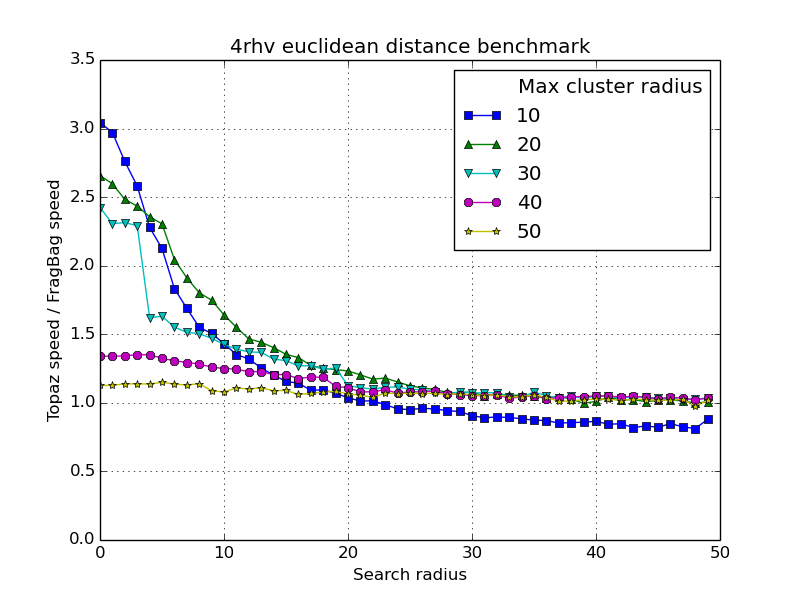
\includegraphics[width=1\textwidth]{assets/4rhv_euclid.png}
    \end{subfigure}
    \begin{subfigure}[b]{0.40\textwidth}
        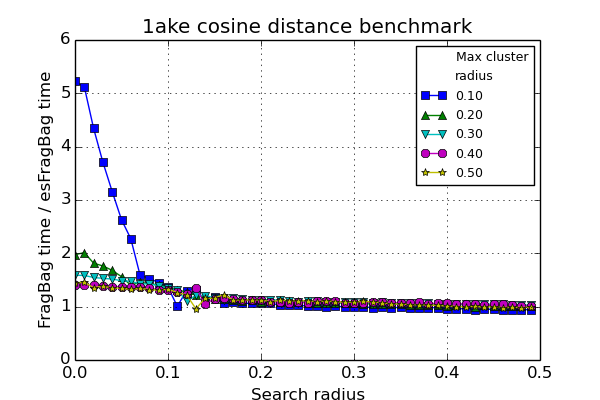
\includegraphics[width=1\textwidth]{assets/1ake_cosine.png}
        %\caption{}
    \end{subfigure}%
    \begin{subfigure}[b]{0.40\textwidth}
        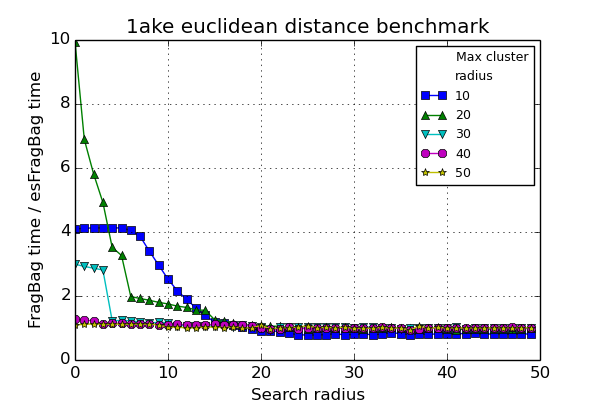
\includegraphics[width=1\textwidth]{assets/1ake_euclid.png}
        %\caption{}
    \end{subfigure}
    \begin{subfigure}[b]{0.40\textwidth}
        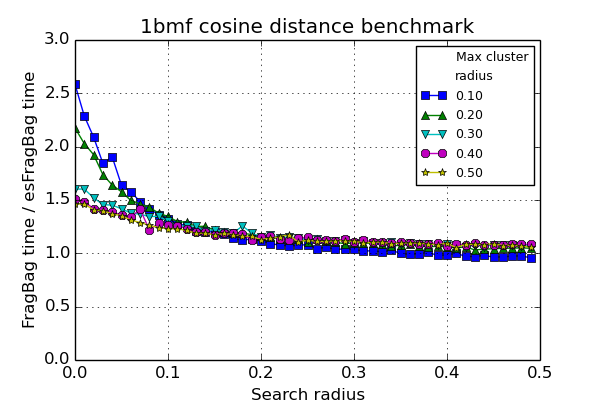
\includegraphics[width=1\textwidth]{assets/1bmf_cosine.png}
        %\caption{}
    \end{subfigure}%
    \begin{subfigure}[b]{0.40\textwidth}
        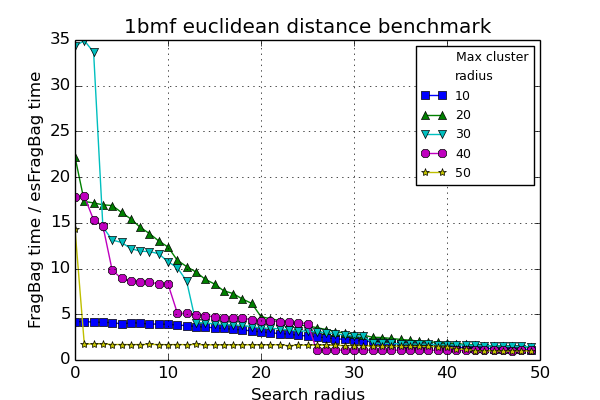
\includegraphics[width=1\textwidth]{assets/1bmf_euclid.png}
        %\caption{}
    \end{subfigure}
    \begin{subfigure}[b]{0.40\textwidth}
        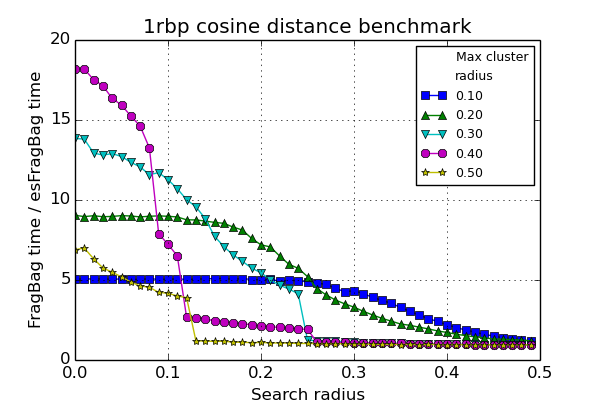
\includegraphics[width=1\textwidth]{assets/1rbp_cosine.png}
        %\caption{}
    \end{subfigure}%
    \begin{subfigure}[b]{0.40\textwidth}
        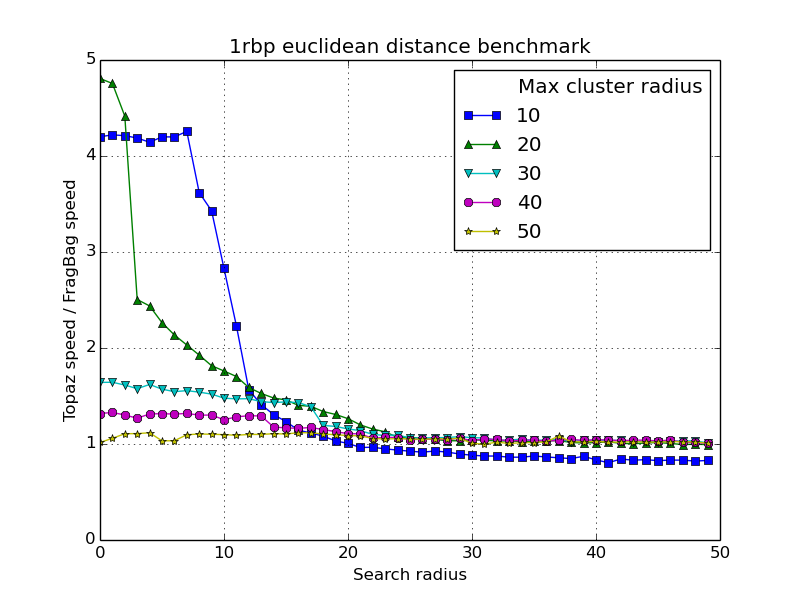
\includegraphics[width=1\textwidth]{assets/1rbp_euclid.png}
        %\caption{}
    \end{subfigure}
    \caption{FragBag benchmarking data with parameters varied until acceleration disappears. As search radius increases, the fraction of the database returned by the coarse search increases, ultimately returning the whole database. Unsurprisingly, when returning the whole database in the coarse search results, there are no benefits to using entropy scaling data structures. (a) Cosine distance gives on the whole better acceleration, but results in only $>99.8\%$ sensitivity, whereas (b) Euclidean distance as a metric is guaranteed by the Triangle Inequality to get $100\%$ sensitivity.}
    \label{fig:fragbag}
\end{figure}

Finally, while Euclidean distance is a metric---for which the triangle inequality guarantees 100\% sensitivity---cosine distance is not.
Empirically, however, for all of the queries we performed, we achieve $> 99.8\%$ sensitivity (Table \ref{tab:fragbag_cosine_sensitivity}).
%Full results for each data point can be found in supplementary data files.

\begin{table}
    \centering
    \caption{Average sensitivity of esFragBag compared to FragBag when using cosine distance for the trials described in Figure \ref{fig:fragbag_cosine}. This table averages the sensitivities for each choice of search radii $\{0, 0.01, \ldots, 0.49\}$. (NB: no analogous table is given for euclidean distance as the Triangle Inequality ensures perfect recall).}
    \label{tab:fragbag_cosine_sensitivity}
    \begin{tabular}{|c|cccc|}
        \hline
        \backslashbox{Cluster radii}{Query protein}  & 4rhv & 1ake & 1bmf & 1rbp \\
        \hline
        0.10  & 1  & 0.999840     & 0.998490 & 0.999950  \\
        0.20  & 1  & 0.999918     & 0.999001 & 0.999978  \\
        0.30  & 1  & 0.999926     & 0.999649 & 1  \\
        0.40  & 1  & 0.999974     & 0.999796 & 1  \\
        0.50  & 1  & 0.999984     & 0.999934 & 1  \\
        \hline
    \end{tabular}
\end{table}

\section{Discussion}

We have introduced a data structure for accelerating approximate search, and
demonstrated its effectiveness in three distinct areas of computational
molecular biology.
This data structure provably scales almost linearly with entropy of the 
database, allowing search on large data sets to scale even as these data sets
grow exponentially.
We provide open-source software for all three areas: caBLASTX for metagenomic analysis,
Ammolite for small-molecule structure search, and esFragBag for protein structure search.
In the case of metagenomic analysis, caBLASTX also compares favorably to recent 
search tools that outperform BLASTX.

In this work, we have not focused on the space-saving compression that is
possible with entropy-scaling data structures, but rather on the run-time
acceleration of approximate search.
However, as discussed in the Supplemental Theory, entropy scaling data structures
allow for compressive algorithms under certain additional constraints.
This is particularly applicable in the case of metagenomic analysis, where the collection of 
read data presents a problem for storage and transfer.
It is worth noting that implementing this compression is feasible using existing software tools and libraries such as BZGF (Blocked GZip).

Entropy-scaling data structures for massive biological data have the great
advantage of becoming proportionately faster and space-efficient with the
size of the available data. Although we have demonstrated their scaling 
behavior for common problems across metagenomics, chemogenomics, and protein
structure search, they can be applied directly or with simple domain
knowledge to a vast array of other problems faced in data science. As
biological data continues to accumulate, entropy-scaling data structures
will become critical to fully realizing the potential of compressive
algorithms for biology. 

\section{Methods}
\subsection{CaBLASTX}

In CaBLASTX, the clustering framework extends the approach of caBLASTP~\cite{daniels2013compressive}.
We augmented the entropy scaling data structure by using
different distance functions for clustering and search.
For clustering, we rely on sequence identity, while for search, we use the
E-value measure that is standard for BLAST.
Furthermore, during clustering (compression), we apply a preprocessing step that
identifies subsequences to be treated as distinct points in the database.
This is because protein sequences commonly contain motifs found in other sequences,
so the natural lexical unit is the motif.
Also during preprocessing, we apply a reversible alphabet reduction to the
protein sequences, which further increases clustering effectiveness (see Supplemental Methods).

As further discussed in Supplemental Methods, when applied to high-coverage next-generation sequencing queries, caBLASTX can also perform clustering on the reads.
In this instance, coarse search is performed by matching each representative query with a set of representative database entries.
Fine search then matches the original queries within each cluster with the candidate database entries resulting from the coarse search.

\subsection{Ammolite}
Our clustering approach relies on structural similarity.
In order to more effectively group molecules based on structural motifs,
each molecule is \emph{simplified} by removing nodes and edges that do not
participate in simple cycles.
Clusters are formed of molecules that are isomorphic after this simplification
step.
Each cluster can then be represented by a single molecular structure, along 
with pointers to \emph{difference sets} between that structure and each of the 
full molecules it represents.
The difference set contains the nodes and edges that were removed in the 
simplification step.

We implemented a variant of a maximum common subgraph (MCS) algorithm, known as 
\emph{flexible} maximum
common subgraph (fMCS), as detailed by Cao, et al.~\cite{cao2008maximum}.
Our implementation allows a user to specify whether any atom mismatches or 
bond-type mismatches should be 
allowed in the maximum common subgraph of two molecules.
If zero mismatches are allowed, fMCS is just MCS.
The distance function used currently is based on the overlap coefficient 
defined as $d(G_1,G_2) = 1 - \frac{ |mcs(G_1,G_2)| }{min(|G_1|,|G_2|)}$. This function, unlike 
the graph distance function  ~\cite{bunke1998graph}, is not a metric. However it does account for
situations where a large molecule contains a smaller molecule which is important in practice.

As in~\cite{loh2012compressive}, our compression-accelerated search approach 
relies on a two-stage process.
First, a \emph{coarse} search is performed in compressed space, by searching 
the coarse database.
The query molecule is simplified in exactly the same manner as 
the molecular database during clustering, and this transformed query graph is 
matched against the coarse database.
To preserve sensitivity, this coarse search is performed with a permissive 
similarity score.
The idea behind coarse search is to identify \emph{possible} hits.


Any possible hits--molecular graphs from the coarse database whose MCS to 
the transformed query molecule was within the similarity score threshold--are 
then reconstructed, by following
pointers to the removed atom and bond information, and recreating the 
original molecules.

Next, the \emph{fine search} is performed against these decompressed possible 
hits.
Fine search is performed using MCS or fMCS, with user-defined parameters for 
bond and atom mismatches and similarity-score threshold.


\subsection{esFragBag}
In FragBag, the bag of fragments is essentially
a term frequency vector representing the number of occurrences of each structural motif within the protein.
While FragBag does not generate structural alignments the way standard aligners do, it provides an excellent
filter for computing proteins that are likely to have close alignments; those alignments could then be computed
with a standard aligner.
FragBag's accuracy has been reported as comparable to structural aligners such as STRUCTAL and
ICE.
FragBag is already quite fast, much faster than these standard aligners, but also importantly for us
FragBag turns out to be very amenable to acceleration using an entropy-scaling data structure because much of the computation is spent in doing a similarity search on a frequency vector.

For the cluster generation, we used a randomized greedy 2-pass approach.
First, all proteins in the Protein Data Bank were randomly ordered.
Then in the first pass, proteins were selected as cluster centers if and only if they were not within a user-specified Euclidean distance $r_c$ from an existing center (i.e. the first protein is always selected, and the second if further away than $r_c$ from the first, etc.).
Recall that this generation of cluster centers is the same as the one used to generate covering spheres in Figure \ref{fig:tree};
the covering spheres were overlapping, but we trivially assign every protein uniquely to a single cluster by assigning to the nearest cluster center in the second pass.

Similarity search here is performed exactly as described in the data structure section, with no modifications.
For a given search query $q$ and search radius $r$,
\begin{itemize}
    \item A coarse search is used to find all cluster centers within distance $r+r_c$ of $q$.
    \item All corresponding clusters were unioned into a set $F$.
    \item A fine search was performed over the set $F$ to find all proteins within distance $r$ of $q$.
\end{itemize}

\section{Author Contributions}
Y.W.Y., N.M.D. and B.B. conceived the project.
Y.W.Y. and B.B. developed the theoretical analyses, with help from N.M.D.
N.M.D. implemented and benchmarked caBLASTX, with help from D.C.D.
D.C.D. implemented and benchmarked Ammolite, with help from N.M.D.
Y.W.Y. applied the entropy-scaling data structure to accelerate FragBag, with help from N.M.D.
B.B. guided all research and provided critical advice on the study.
Y.W.Y., N.M.D. and B.B. wrote the manuscript.

\section{Acknowledgments}
Y.W.Y. is supported by a Hertz Foundation fellowship.
N.M.D. and B.B. are supported by NIH GM108348.
We thank Andrew Gallant for his implementation of Fragbag.
We thank Jian Peng for suggesting high-throughput drug screening as an application.

\bibliographystyle{model5-names-noitalic}
%\bibliographystyle{plain}
\bibliography{main}

\end{document}

